\hsection{Iteration, Comprehension, and Generators}%
\label{sec:iteration}%
%
In \python, iterating over the items in a sequence is a central concept.
In \cref{sec:enumOverSequences}, we learned that we can iterate over collections such as lists, tuples, dictionaries, and sets.
We can also iterate over the characters in a string in the same way.
These are all datastructures whose complete content exists in memory at any given time.
In \python, we can also iterate over sequences where the items that are constructed at the time when they are actually needed.
A good example for this is the \pythonilIdx{range} datatype.
We can iterate over all the 1'000'000'000 \pythonil{int} elements of \pythonil{range(1_000_000_000)} in a loop.
These many integers do not all exist in memory at the same time.
Instead, they are provided one-by-one as needed.
From the perspective of a programmer, we can iterate over a \pythonilIdx{range} and a \pythonilIdx{list} in exactly the same way.
Matter of fact, many objects in \python\ support iteration.

Vice versa, we can also create container datatypes from sequences of items.
For example, the datatypes \pythonilIdx{list}, \pythonilIdx{tuple}, \pythonilIdx{set}, and \pythonilIdx{dict} can also be used like functions that take a sequence of items as parameter and create in instance of the corresponding datatype.
In \cref{sec:lists:basicFunctions}, we learned that \pythonil{[1, 2, 2, 3]} creates a list with the specified contents.
Passing this list to the \pythonilIdx{set} function/datatype, i.e., writing \pythonil{set([1, 2, 2, 3])} will create the set \pythonil{\{1, 2, 3\}}.
We also learned that we modify several datastructures in place by combining them with other containers.
Invoking \pythonil{l.extend(\{1, 2, 3\})}\pythonIdx{list!extend}\pythonIdx{extend} will append the elements~\pythonil{1}, \pythonil{2}, and \pythonil{3} to a list~\pythonil{l}, for example.

\begin{figure}%
\centering%
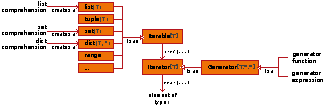
\includegraphics[width=0.96\linewidth]{\currentDir/iteration.pdf}%
\caption{The concepts of comprehension, \pythonilsIdx{Iterable}, \pythonilsIdx{Iterator}, and \pythonilsIdx{Generator} in \python.}%
\label{fig:iteration}%
\end{figure}%

Much later -- in a chapter that I have not yet written -- we learn that we also can iterate over the contents of a file.
You will very often encounter situations where you transform, process, or create sequences of data elements.
As sketched in \cref{fig:iteration}, there are many different manifestations of the concepts of \emph{iterating} over objects that are \emph{iterable} in \python.
In this chapter, we will investigate those that we did not yet already discuss in \cref{sec:enumOverSequences,sec:collections}.
%
\hsection{\texttt{Iterable}s and \texttt{Iterator}s}%
\label{sec:iterable}%
%
\begin{figure}%
\centering%
%
\subfloat[][%
Manually iterating over a \pythonilIdx{list}.%
\label{fig:iterateOverListAndRange:list}%
]{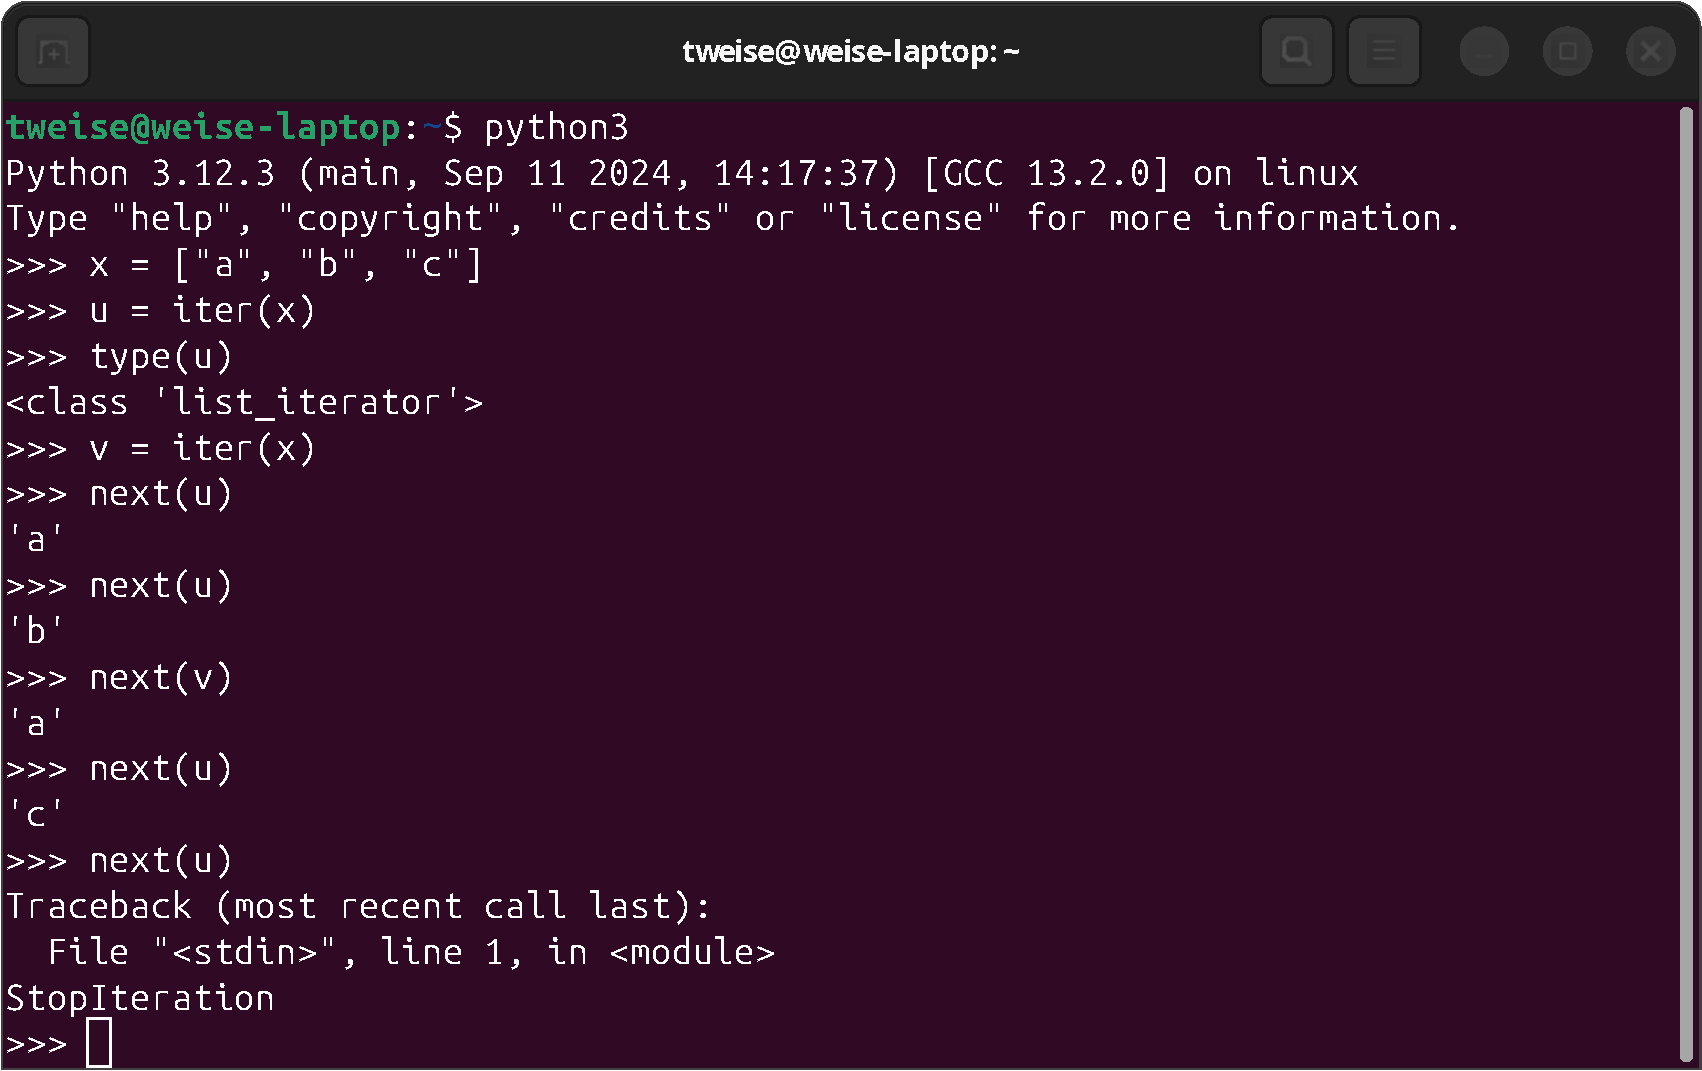
\includegraphics[width=0.7\linewidth]{\currentDir/listIterConsole}}%
%
\\[12pt]%
%
\subfloat[][%
Manually iterating over a \pythonilIdx{range}.%
\label{fig:iterateOverListAndRange:range}%
]{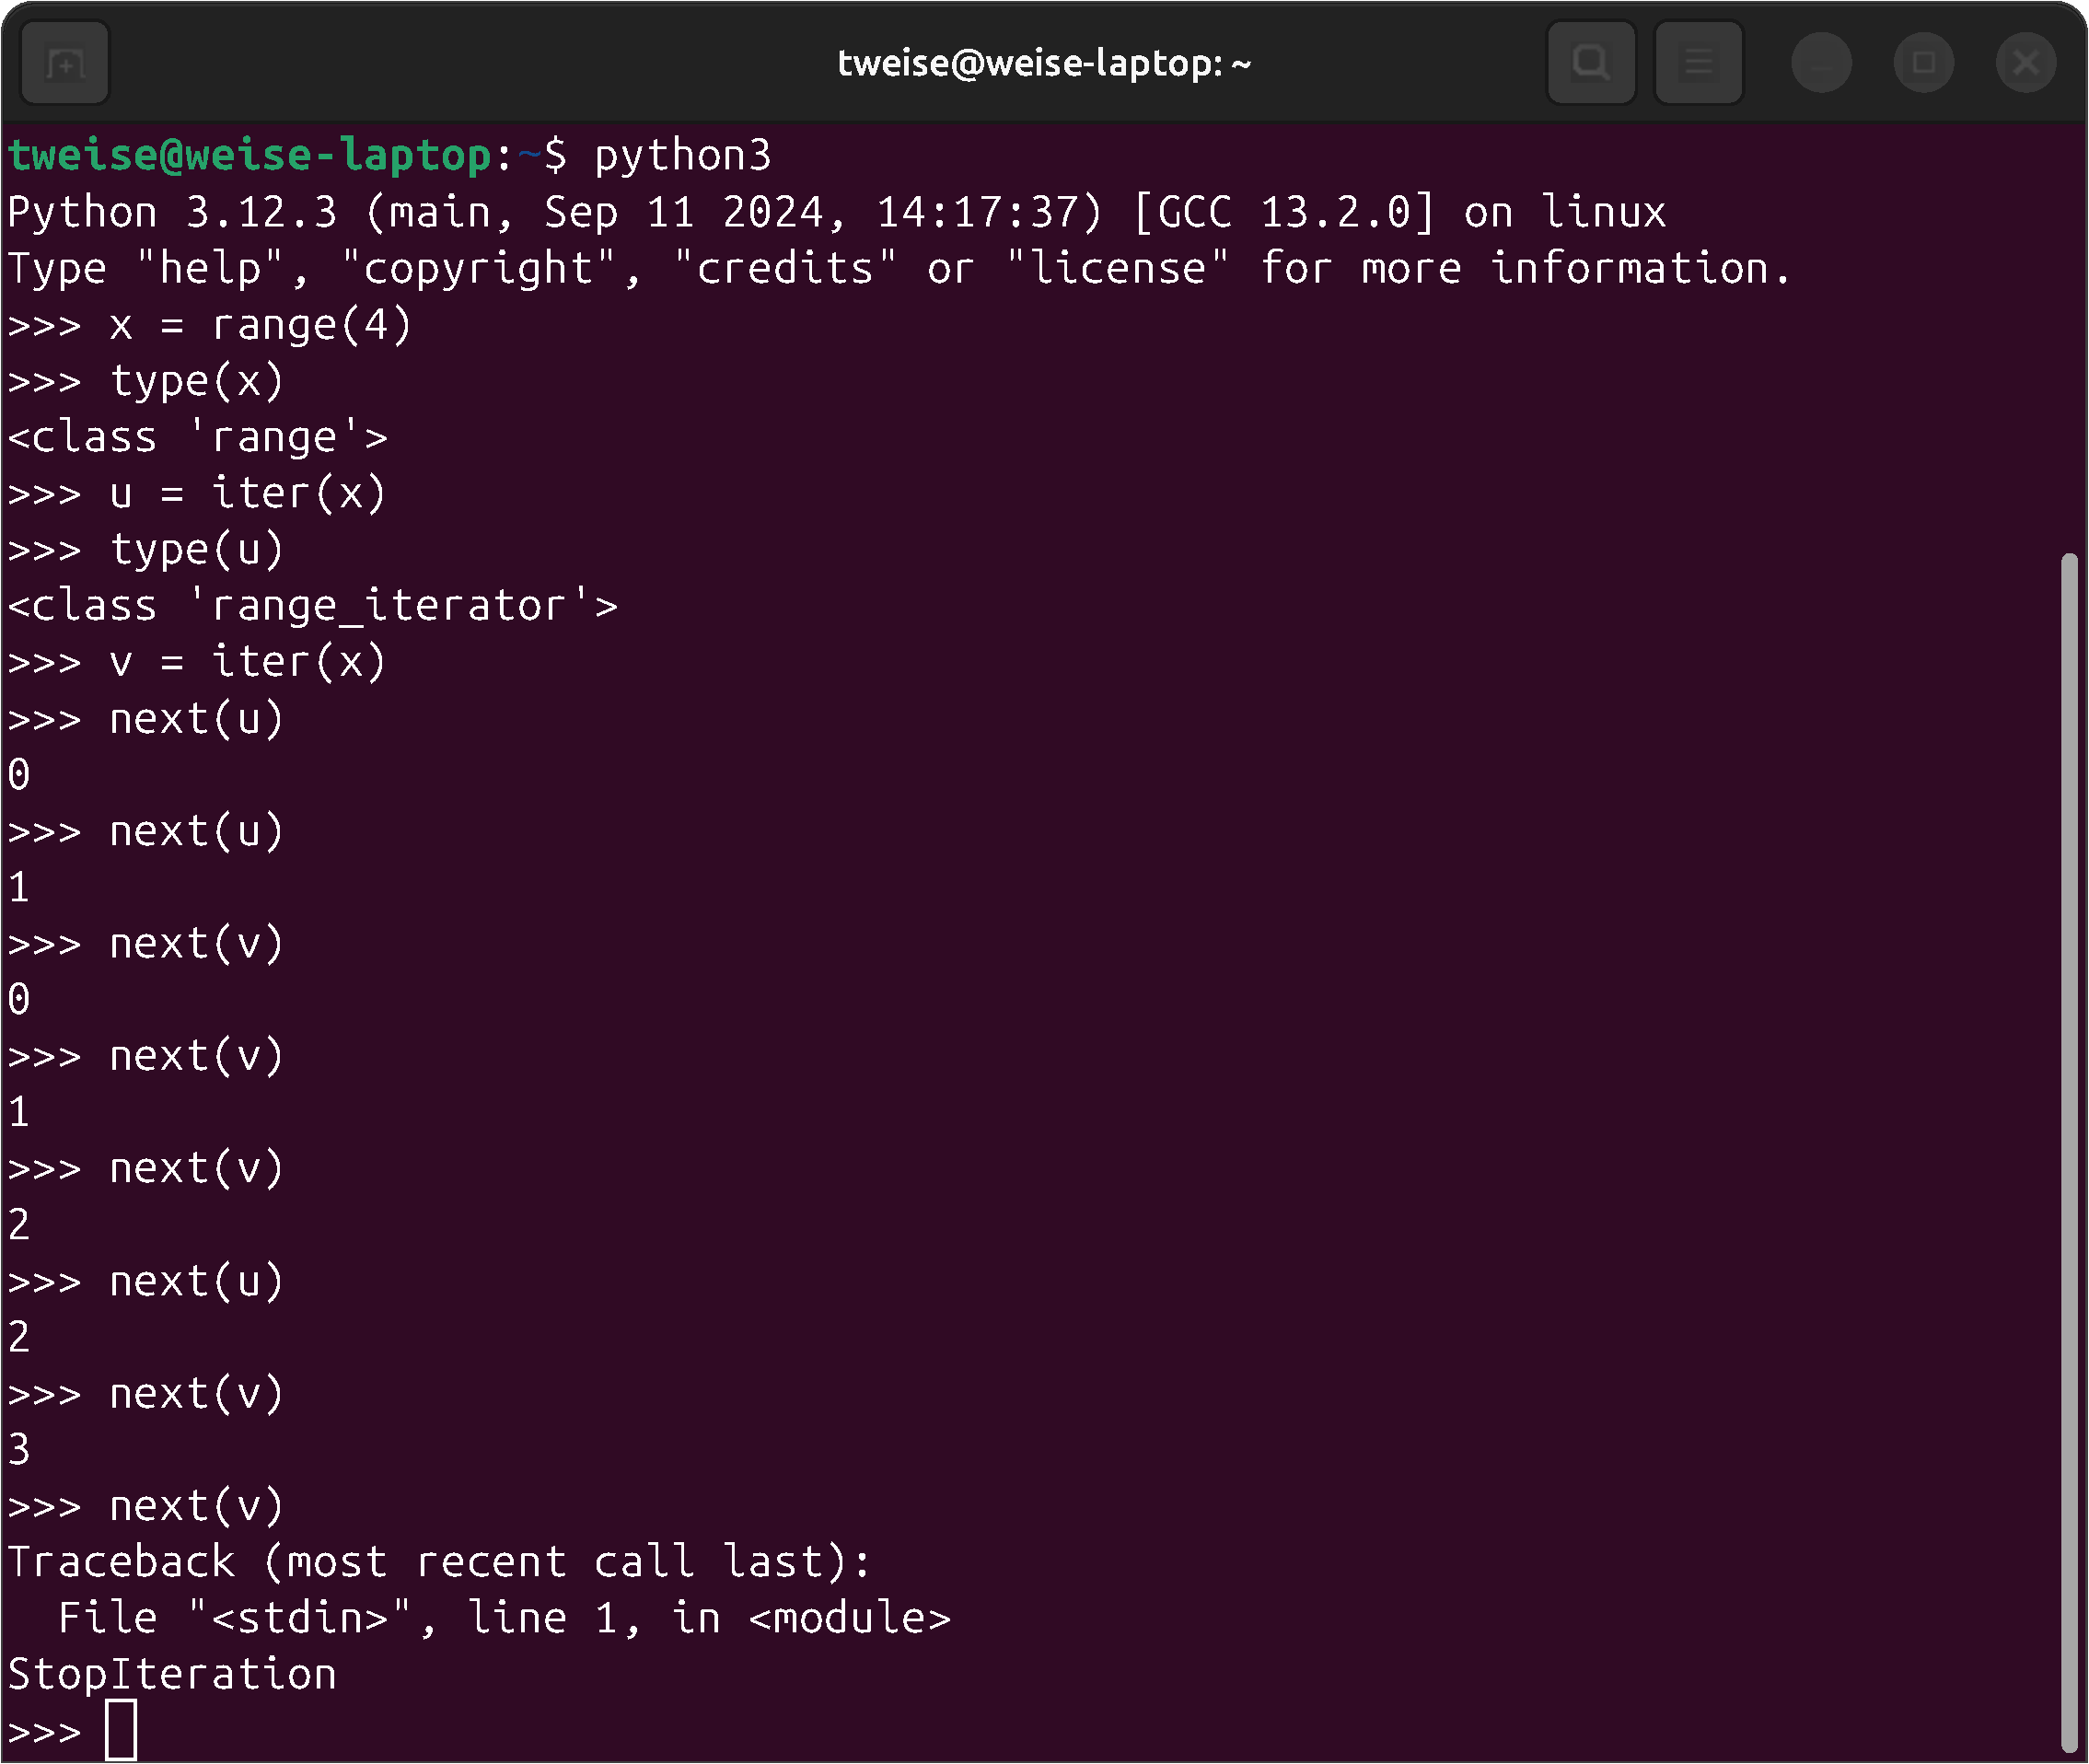
\includegraphics[width=0.7\linewidth]{\currentDir/rangeIterConsole}}%
%
%
\caption{Manually iterating over a \pythonilIdx{list} and a \pythonilIdx{range} in the \python~console.}%
\label{fig:iterateOverListAndRange}%
\end{figure}%
%
\begin{sloppypar}%
Any object that allows us to access its elements one-by-one, i.e., \emph{iteratively} is an instance of \pythonilIdx{typing.Iterable}\pythonIdx{Iterable}.
The actual iteration over the contents is then done by an \pythonilIdx{typing.Iterator}\pythonIdx{Iterator}.
This distinction is necessary because we want to allow some objects to be iterated over multiple times.%
\end{sloppypar}%
%
Let's say you have the list \pythonil{x = ["a", "b", "c"]}, as in \cref{fig:iterateOverListAndRange:list}.
We can use this list~\pythonil{x} in a \pythonil{for xi in x}-kind of loop arbitrarily often.
\pythonil{x} is an instance of \pythonilIdx{list} and every list is also an~\pythonilIdx{Iterable}\pythonIdx{typing.Iterable}.
Every time we do loop over \pythonil{x}, an \pythonilIdx{Iterator} instance is created internally by (doing something like) invoking~\pythonil{y = iter(x)}\pythonIdx{iter}.
In principle, this \pythonilIdx{Iterator} object only has to remember its current position in the list, allowing us to query the next item by invoking~\pythonil{next(y)}\pythonIdx{next}.
The \pythonilIdx{for}-loop basically does this internally.
However, we can also do it \inQuotes{by hand.}
In \cref{fig:iterateOverListAndRange:list}, we perform \pythonil{u = iter(x)} and \pythonil{v = iter(x)}.
This creates two independent \pythonilsIdx{Iterator}, which we can use to step over the list separately.
Invoking \pythonil{next(u)}\pythonIdx{next} will yield the first element of the list~\pythonil{x}, namely~\pythonil{"a"}.
Calling \pythonil{next(u)}\pythonIdx{next} again gives us the second element, that is~\pythonil{"b"}.
If we now call \pythonil{next(v)}\pythonIdx{next}, i.e., apply~\pythonilIdx{next} to the second, independent \pythonilIdx{Iterator}, we again obtain the first element~(\pythonil{"a"}).

This shows us why there is a distinction between \pythonilIdx{Iterable} and \pythonilIdx{Iterator}.
The former is the object that holds or can generate the data sequence.
The latter marks one independent iteration over that sequence.

The third invocation of \pythonil{next(u)}\pythonIdx{next} gives us~\pythonil{"c"}, the third and last element of~\pythonil{x}.
If we now call \pythonil{next(u)}\pythonIdx{next} a fourth time, something interesting happens:
A \pythonilIdx{StopIteration} is raised\pythonIdx{raise}.
This is not an error in the strict sense.
This instead is how the end of an iteration sequence is signaled.
A \pythonilIdx{for}~loop will, for instance, stop when it encounters this exception.

This approach to iterate over collections by first creating an iterator using the \pythonilIdx{iter} function and then applying \pythonilIdx{next} to that iterator works for \pythonilsIdx{list} and \pythonilsIdx{tuple} alike.
It also works for \pythonilsIdx{set}, but be aware that the order in which the elements of a \pythonilIdx{set} are presented is not defined.
Back in \cref{bp:setsUnordered} we already clarified that \pythonilsIdx{set} are unordered data structures.
Interestingly, we can also iterate over \pythonilsIdx{dict} like this.
This iteration \emph{only} returns the dictionary keys however.
If we need the values or the key-value pairs of a dictionary~\pythonil{d}, then we have to iterate over \pythonil{d.values()}\pythonIdx{values}\pythonIdx{dict.values} or \pythonil{d.items()}\pythonIdx{items}\pythonIdx{dict.items}, respectively.

\Cref{fig:iterateOverListAndRange:range} shows us that even \pythonilsIdx{range} have the exactly same behavior as \pythonilsIdx{list} with respect to iteration.
And they should, of course, like every other object implementing the~\pythonilIdx{Iterable} functionality.
Because of this, the \pythonil{for y in x}-type of loops can be applied to any \pythonilIdx{Iterable} or \pythonilIdx{Iterator} instance~\pythonil{x}.%
%
\endhsection%
%
\hsection{List Comprehension}%
%
We can create a list by writing it down as a literal, e.g., \pythonil{[1, 2, 3, 4, 5]} creates a list\pythonIdx{list} containing the first five natural numbers.
This is very handy, but can also become cumbersome if we either have many elements or want to transform them.
Needing to write a literal in the same way that creates a list with the first one hundred natural numbers may be somewhat annoying.
If we want to create a list with the logarithms of first five natural numbers, writing \pythonil{[log(1), log(2), log(3), log(4), log(5)]}\pythonIdx{log} looks clunky as well.
Luckily, \python\ offers the much more convenient syntax of list comprehension\pythonIdx{list!comprehension}\pythonIdx{comprehension!list}~\cite{PEP202}:%
%
\begin{pythonSyntax}
# Create a list from the items in a sequence; the condition is optional
[expression for item in sequence if condition]
\end{pythonSyntax}
%
\gitPythonAndOutput{\programmingWithPythonCodeRepo}{07_iteration}{simple_list_comprehension.py}{--args format}{iteration:simple_list_comprehension}{%
Some simple examples for list comprehension\pythonIdx{list!comprehension}\pythonIdx{comprehension!list}.}%
%
\gitOutputTool{\programmingWithPythonCodeRepo}{.}{scripts/ruff.sh 07_iteration simple_list_comprehension.py}{iteration:simple_list_comprehension:ruff}{%
The output of \ruff\ for the examples for list comprehension in \cref{lst:iteration:simple_list_comprehension}: %
The \pythonilIdx{for}~loop constructing the list \textil{squares_1} can indeed by replaced by a list comprehension\pythonIdx{list!comprehension}\pythonIdx{comprehension!list}.}%
%
\begin{sloppypar}%
This syntax creates a new list whose contents are the results of applying a given \pythonil{expression} to the items~\pythonil{item} from another \pythonil{sequence}.
For example, \pythonil{[i for i in range(10)]} creates a list with the integer numbers~\pythonil{0} to~\pythonil{9}.
The comprehension \pythonil{[i ** 2 for i in range(10)]} instead creates a list with their squares (where \inQuotes{squaring} is the before-mentioned expression).
Additionally, we can select the elements that we want to have in the list by adding an \pythonilIdx{if}~clause:
\pythonil{[i for i in range(10) if i != 3]}, for instance, excludes the number~\pythonil{3} from our list.
Interestingly, the sequence over which the list creation iterates can itself also be such a comprehension expression.
It is totally fine to write \pythonil{[i * j for i in range(2) for j in range(2)]}, which yields \pythonil{[0, 0, 0, 1]} because both~\pythonil{i} and~\pythonil{j} will take on the values~\pythonil{0} and~\pythonil{1}.%
\end{sloppypar}%
%
In \cref{lst:iteration:simple_list_comprehension} we provide some examples for list comprehension.
First, we want to construct a list with the squares of the integer numbers from~0 to~10.
Before learning about list comprehension, we would do this by initially creating an empty list~\pythonil{squares_1}.
In a \pythonilIdx{for}~loop letting a variable~\pythonil{i} iterate over the \pythonil{range(0, 11)}\pythonIdx{range}, we would then add \pythonil{i ** 2} to the list~\pythonil{squares_1} by invoking~\pythonil{squares_1.append(i ** 2)}\pythonIdx{list!append}\pythonIdx{append}.
This will occupy at least three lines of code.
Instead, we could write the comprehension expression \pythonil{[j ** 2 for j in range(11)]}, which achieves exactly the same thing only using a single line of code.

We can also select which elements we want to insert into our list by using an \pythonilIdx{if} statement during the list comprehension.
In \cref{lst:iteration:simple_list_comprehension}, we demonstrate this by creating a list of even numbers from the range~0 to~9.
We let a variable~\pythonil{k} iterate over the \pythonil{range(10)}\pythonIdx{range}.
This lets~\pythonil{k} take on the values~\pythonil{0}, \pythonil{1}, \pythonil{2}, \dots, \pythonil{8}, and finally~\pythonil{9}.
Out of these values, we select only those for which \pythonil{k \% 2 == 0} via the \pythonilIdx{if}~statement.
In other words, we compute the result of the \pgls{modulodiv} of \pythonil{k} and~\pythonil{2}, i.e., the remainder of that division.
If it is zero, then \pythonil{k} is divisible by~\pythonil{2} and thus even.
Anyway, we obtain the list~\pythonil{[0, 2, 4, 6, 8]}.%
%
\begin{sloppypar}%
Finally, we play around with \inQuotes{nested} comprehension.
Let's say you have two \pythonilsIdx{Iterable} and want to produce all possible combinations of their output.
Assume that the first sequence by~\pythonil{"abc"} and the second one be~\pythonil{"xy"}.
How can we achieve this?
By simply writing two \pythonil{for}~statements!
In \cref{lst:iteration:simple_list_comprehension}, we create the list~\pythonil{combinations} this way.
We write \pythonil{[f"\{m\}\{n\}" for m in "abc" for n in "xy"]}.
This lets the variable~\pythonil{m} take on all the characters in the string~\pythonil{"abc"}.
For each of the values that~\pythonil{m} takes on, the variable~\pythonil{n} iterates over \pythonil{"xy"} and thus first becomes~\pythonil{"x"} and then~\pythonil{"y"}
The \pgls{fstring} \pythonil{f"\{m\}\{n\}"} is extrapolated for each combination of~\pythonil{m} and~\pythonil{n}.
The result is thus the list~\pythonil{["ax", "ay", "bx", "by", "cx", "cy"]}.%
\end{sloppypar}%
%
\begin{sloppypar}%
Of course, we can create lists of arbitrary datatypes using list comprehension.
These include also other lists, tuples, sets, dictionaries -- whatever we want.
We can repeat the above example and, instead of storing the combinations of characters as strings, we could store them as \pythonilsIdx{tuple}.
The list comprehension~\pythonil{[(o, p) for o in "abc" for p in "xy"]} does this.
It produces~\pythonil{[('a', 'x'), ('a', 'y'), ('b', 'x'), ('b', 'y'), ('c', 'x'), ('c', 'y')]}.
\end{sloppypar}%
%
In \cref{exec:iteration:simple_list_comprehension:ruff}, we present the output that \ruff, our \cref{ut:ruff}, produces when we apply it to \cref{lst:iteration:simple_list_comprehension}.
Interestingly, \ruff\ considers the construction of a list via the \pythonilIdx{append}\pythonIdx{list!append} function as a \emph{performance issue}, signified by the error prefix~\textil{PERF}.
This is, of course, only the case if the list could as well be created via list comprehension, which is not always possible.
But when it can be done, as is the case in our example, we noticed that list comprehension is more compact.
Code which is more compact is often more readable and in this case, from a software engineering point of view, preferable.
But why would this also be an issue of performance, i.e., execution speed?

\gitPythonAndOutput{\programmingWithPythonCodeRepo}{07_iteration}{list_of_numbers_append.py}{--args format}{iteration:list_of_numbers_append}{%
Create a \pythonilIdx{list} with the even numbers from~0 to~1'000'000 using the \pythonilIdx{append}.}%
%
\gitPythonAndOutput{\programmingWithPythonCodeRepo}{07_iteration}{list_of_numbers_comprehension.py}{--args format}{iteration:list_of_numbers_comprehension}{%
Create a \pythonilIdx{list} with the even numbers from~0 to~1'000'000 using list comprehension.}%

In order to investigate this issue, we could try to simply create two lists with the same contents, once by using the \pythonilIdx{append} method and once by using list comprehension.
Whichever is faster, i.e., needs less time, has the better performance.
Now measuring the runtime needed by something is always a dodgy subject.
The runtime of a \python\ interpreter obviously depends on the machine and CPU it is running on.
It is also affected by the operating system, the available RAM, the disk speed, and of course by other processes running on the same machine at the same time.
Clearly, it also depends on which version of the \python\ interpreter we use and our results could be different after each software update.
So every runtime measurement is always fuzzy and imprecise.
Whatever we would measure would have to take with a grain of salt, but we will try it anyway.%
%
\usefulTool{timeit}{%
\pythonilIdx{timeit} is a tool for measuring execution time of small code snippets that ships directly with \python. %
This module avoids a number of common traps for measuring execution times, see~\cite{PSF2024TMETOSCS,P2002AI}.%
}%
%
\pythonilIdx{timeit} allows us to measure the runtime of a certain statement.
We want to measure how long it takes to create a list containing all even numbers from~0 to~1'000'000.

In \cref{lst:iteration:list_of_numbers_append} we therefore first implement a function \pythonil{create_by_append} which constructs the list using the \pythonilIdx{append}\pythonIdx{list!append} method.
In a loop over the \pythonil{range(1_000_001)}, it appends all the even numbers to the list \pythonil{numbers}.
Finally, it returns the list.

To measure the runtime of this function, we first \pythonilIdx{import} the function \pythonilIdx{repeat}\pythonIdx{timeit!repeat} from the module~\pythonilIdx{timeit}.
We tell \pythonilIdx{repeat} to call our function \pythonil{create_by_append} one time and measure the consumed runtime (which will be in seconds and stored in a \pythonil{float}).
However, due to the above factors which may influence the runtime, a single measurement is not very reliable~\cite{P2002AI}.
We thus instruct \pythonilIdx{repeat} to take 90 such measurements.
All of the measured runtimes are then return as a \pythonil{list[float]}.
The documentation of \pythonilIdx{timeit}~\cite{PSF2024TMETOSCS} says:%
%
\begin{quote}%
\emph{Note:}~it's tempting to calculate mean and standard deviation from the result vector and report these.
However, this is not very useful.
In a typical case, the lowest value gives a lower bound for how fast your machine can run the given code snippet;
higher values in the result vector are typically not caused by variability in \python's speed, but by other processes interfering with your timing accuracy.
So the \pythonil{min()}\pythonIdx{min} of the result is probably the only number you should be interested in.
After that, you should look at the entire vector and apply common sense rather than statistics.%
\end{quote}%
%
\bestPractice{timeMeasurement}{%
When measuring the runtime of code for one specific set of inputs, it makes sense to perform multiple measurements and to take the \emph{minimum} of the observed values~\cite{PSF2024TMETOSCS}. %
The reason is that there are many factors (CPU temperature, other processes, \dots) that may \emph{negatively} impact the runtime. %
However, there is no factor that can make your code faster than what your hardware permits. %
So the minimum is likely to give the most accurate impression of how fast your code can theoretically run on your machine. %
Notice, however, that there might be effects such as caching that could corrupt your measurements.%
}%
%
So we do just that.
We print the result of \pythonilIdx{min} applied to the returned list.
We format the output to be in milliseconds and rounded to three digits, to be a bit more readable.
The result can be seen in \cref{exec:iteration:list_of_numbers_append}.

Now the PDF of this book is built automatically using a \github~Action~\cite{C2024GA}.
This action executes all the \python\ example programs and weaves their output into the book.
Everytime I update the book, this process is repeated.
This means that, when writing this text, I do not know what value you will see in \cref{exec:iteration:list_of_numbers_append}.
On my local machine, I get \textil{runtime/call: 30.1 ms.}

Anyway, in order to test whether list comprehension is really faster than iterative list construction via \pythonilIdx{append}\pythonIdx{list!append}, we now write the second program \cref{lst:iteration:list_of_numbers_comprehension}.
This program is very similar to \cref{lst:iteration:list_of_numbers_append}.
It defines a function \pythonil{create_by_comprehension} which creates the very same list as \pythonil{create_by_append} does in \cref{lst:iteration:list_of_numbers_append}.
However, it uses list comprehension.
We measure the runtime of this function in exactly the same way as before.
In \cref{exec:iteration:list_of_numbers_comprehension}, you can see the result.
Of course, this result may be different every time the book is compiled using the \github~Action mentioned above.
On my local machine, I get \textil{runtime/call: 28.7 ms.}

This confirms that list comprehension is indeed a bit faster than iterative list construction on \python~3.12.
The difference may have been bigger on older \python\ versions, but it is there.
Five percent of runtime saved are nice.
And even if list comprehension was not faster than iteratively constructing a list, it would still be better code, because it is shorter and more readable.%
%
\FloatBarrier%
\endhsection%
%
\hsection{Brief Interlude: doctests}%
\gitPython{\programmingWithPythonCodeRepo}{07_iteration/list_flatten_iterables.py}{--args format}{iteration:list_flatten_iterables}{%
A function that flattens \pythonilsIdx{list} and other \pythonilsIdx{Iterable} using list comprehension.}%
%
\gitOutputTool{\programmingWithPythonCodeRepo}{.}{scripts/pytest_doctest.sh 07_iteration list_flatten_iterables.py}{iteration:list_flatten_iterables:doctest}{%
The output of \pytest\ executing the \pglspl{doctest} for the examples for list comprehension in \cref{lst:iteration:list_flatten_iterables}: %
The test succeeded. %
We used the test execution script given in \cref{lst:bash:pytest_doctest}.}%
%
As last example for list comprehension, let us consider the following scenario:
Let's say that you have several different lists.
You want to create a new list that contains all the elements of each of these existing lists.
In \cref{lst:iteration:list_flatten_iterables}, we implement a function~\pythonil{flatten} that achieves an even more general variant of this task:
You can pass in an \pythonilIdx{Iterable} of other \pythonilsIdx{Iterable}.
Since \pythonilsIdx{lists} are \pythonilsIdx{Iterable}, this allows you to pass in a \pythonilIdx{list} of \pythonilsIdx{lists}.
But you could also pass a \pythonilIdx{tuple} of \pythonilsIdx{set} if you want.
The return value of \pythonil{flatten} is a \pythonilIdx{list} containing the elements of all of the \inQuotes{inner} \pythonilsIdx{Iterable}.%
%
\begin{sloppypar}%
\pythonil{flatten} creates this list from its parameter~\pythonil{iterables} by simply returning \pythonil{[value for subiterable in iterables for value in subiterable]}.
The variable \pythonil{subiterable} iterates over \pythonil{iterables}, i.e., becomes one of the, e.g., sub-list, at a time.
Then, \pythonil{value} iterates over the elements of \pythonil{subiterable}.
Thus, it iteratively takes on each of the values in each of the sub-list.
Since we return a \pythonilIdx{list} with all of these values, we effectively flatten the list.
It may be a bit confusing that the inner \pythonilIdx{for}-loop here is actually the outer \pythonilIdx{for}-loop and vice-versa, but we experienced this already when we computed \pythonil{[f"\{m\}\{n\}" for m in "abc" for n in "xy"]}. in an earlier example.%
\end{sloppypar}%
%
Normally, we would also provide some code that actually executes \pythonil{flatten} and present its output.
This time, we do something else:
We present \pglspl{doctest} for \pythonil{flatten}.

\usefulTool{doctest}{%
A \pgls{doctest} is a unit test written directly into the \pgls{docstring} of a function or module. %
We therefore insert small snippets of \python\ code and their expected output. %
The first line of such codes is prefixed py~\pythonil{>>>}\pythonIdx{>\strut>\strut>}. %
If the snipped has multiple lines, any following line is prefixed by~\pythonil{...}\pythonIdx{\idxdots}. %
After the snippet, the expected output is written. %
The \pglspl{doctest} can be by modules like \pythonilIdx{doctest}~\cite{PSF2024DTIPE} or tools such as \pytest~\cite{KPDT2024HTRD}~(\cref{ut:pytest}). %
They collect the code, run it, and compare its output to the expected output in the \pgls{docstring}. %
If they do not match, the tests fail. %
We use \pytest\ in this book, with the default configuration given in \cref{lst:bash:pytest_doctest}.%
}
%
Using \pglspl{doctest} has a very unique advantage:
It allows us to include examples of how our code should be used directly into the \pglspl{docstring}.
And these examples can directly serve as unit tests!
Let's read the \pglspl{docstring} of our \pythonil{flatten} function in \cref{lst:iteration:list_flatten_iterables}.

The first \pgls{doctest} tells us that if we invoke \pythonil{flatten([[1, 2, 3], [4, 5, 6]])}, we can expect the output \pythonil{[1, 2, 3, 4, 5, 6]}.
In other words, our function will flatten the list of two lists into a single list.
Then, we see that \pythonil{flatten([[1, 2, 3], [], [4, 5, 6]])} should produce \pythonil{[1, 2, 3, 4, 5, 6]} as well.
The single empty list in the list-of-lists disappears, because it has no elements.

\pythonil{flatten} can only reduce two list levels to one.
Passing a list-of-lists-of-lists to \pythonil{flatten} as in the third test~(\pythonil{flatten([[[1], [2], [3]], [], [[4], [5], [6]]])}) will only remove one list level.
It results in a list-of-lists~(\pythonil{[[1], [2], [3], [4], [5], [6]]}).%
%
\begin{sloppypar}%
Since \pythonil{flatten} works with \pythonilsIdx{Iterable}, it also accepts mixed input.
The final \pgls{doctest} symbolizes this as follows:
For \pythonil{flatten(([1, 2, 3], (4, 5, 6), {"a": 7, "b": 8}))}, we get \pythonil{[1, 2, 3, 4, 5, 6, 'a', 'b']} as the result.
\end{sloppypar}%
%
As you can see, the documentation in form of examples also explains what output we should expect.
We now execute \pytest\ with the additional option \textil{--doctest-modules}.
The output in \cref{exec:iteration:list_flatten_iterables:doctest} shows that our function indeed fulfills the requirements imposed by its \pglspl{doctest}.%
%
\bestPractice{doctest}{%
Where ever possible, the \pglspl{docstring} of functions and modules should contain \pglspl{doctest}. %
This provides unit tests as well as examples as how the code should be used. %
Since \pglspl{doctest} are usually brief, they are a quick and elegant way to complement more comprehensive unit tests in separate files (see \cref{bp:functionUnitTest}).%
}%
%
\FloatBarrier%
\endhsection%
%
\hsection{Set Comprehension}%
%
Set comprehension works very much the same as list comprehension.
The corresponding syntax is as follows:%
%
\begin{pythonSyntax}
# Create a set from the items in a sequence; the condition is optional
{expression for item in sequence if condition}
\end{pythonSyntax}
%
\gitPythonAndOutput{\programmingWithPythonCodeRepo}{07_iteration}{simple_set_comprehension.py}{--args format}{iteration:simple_set_comprehension}{%
Some simple examples for set comprehension\pythonIdx{set!comprehension}\pythonIdx{comprehension!set}.}%
%
In \cref{lst:iteration:simple_set_comprehension}, we provide some simple examples for set comprehension\pythonIdx{set!comprehension}\pythonIdx{comprehension!set} and in \cref{exec:iteration:simple_set_comprehension} you can find the output of the program.
First, we create a set with the results of the \pythonilIdx{isqrt} function from the \pythonilIdx{math} module.
This function computes the integer part of a square root, i.e., $\pythonil{isqrt(i)}=\left\lfloor\sqrt{\pythonil{i}}\right\rfloor$.
We want to create the set with all results of this function for the values~\pythonil{i} from~0 to~99.
We first do this by starting with an empty set~\pythonil{roots_1} and then iteratively append the values by calling \pythonil{roots_1.add}\pythonIdx{set!add} in a \pythonilIdx{for}-loop.
The constructed set contains, obviously, the values~0 to~9.
Each value is contained a single time, because this is how sets work.%
%
\begin{sloppypar}%
We now create the same set using set comprehension\pythonIdx{set!comprehension}\pythonIdx{comprehension!set}.
The set \pythonil{roots_2} created by evaluating \pythonil{\{isqrt(j) for j in range(100)\}} is exactly the same as \pythonil{roots_1}.
Set comprehension works exactly like list comprehension, and our first examples are also almost the same.%
\end{sloppypar}%
%
Let us now try do something more interesting:
We want to create the set \pythonil{primes} of the prime numbers in the range~2 to~99.
We already created a beautiful program doing this efficiently in \cref{lst:loops:for_loop_sequence_primes}.
This time, we will use set comprehension\pythonIdx{set!comprehension}\pythonIdx{comprehension!set}.

We first compute the set of numbers that are \emph{not} prime.
For this purpose, we let a variable~\pythonil{k} iterate from~\pythonil{2} to~\pythonil{99}.
For each value of~\pythonil{k}, a second variable~\pythonil{m} iterates from~\pythonil{2} to~\pythonil{k - 1}.
For every single one of the resulting \pythonil{k}\nobreakdashes-\pythonil{m} combinations, we will add the value of~\pythonil{k} to the set \emph{if} the condition \pythonil{k \% m == 0} is met.
In other words, every single time we find a number~\pythonil{m} that can divide~\pythonil{k} without remainder, we will insert~\pythonil{k} into the set.
If we would be doing a list comprehension, this would yield a huge list where many values of~\pythonil{k} appear repeatedly.
However, we are doing set comprehension, so each value can occur at most once.%
%
\begin{sloppypar}%
This extremely computationally inefficient gives us the set~\pythonil{not_primes}.
If a number can be divided by another one which is larger than~1 and smaller than the number itself, then it can obviously not be a prime number.
Having the numbers which are not primes, we can now use a second set comprehension to get the numbers which are primes.
\pythonil{\{n for n in range(2, 100) if n not in not_primes\}}\pythonIdx{not in} lets a variable~\pythonil{n} again iterate from~2 to~99.
It includes each value of~\pythonil{n} in the set to be constructed if \pythonil{n} is not in the set \pythonil{not_primes}.
Indeed, this yields the set of prime numbers correctly (but does in a very inefficient way).%
\end{sloppypar}%
%
\FloatBarrier%
\endhsection%
%
\hsection{Dictionary Comprehension}%
%
Dictionary comprehension\pythonIdx{dict!comprehension}\pythonIdx{comprehension!dict} works almost the same as set and list comprehension~\cite{PEP274}.
Different from them, it assigns values to keys and therefore has two expressions denoting each entry, separated by~\pythonilIdx{:}.
This is also the difference between the syntax of set and dictionary comprehension.
Both of them use curly braces, but in dictionary comprehension\pythonIdx{dict!comprehension}\pythonIdx{comprehension!dict}, keys and values are separated by~\pythonilIdx{:}, whereas in a set comprehension, only single values are given.
Dictionary comprehension has the following syntax:%
%
\begin{pythonSyntax}
# Create a dict from the items in a sequence; the condition is optional
{expression1: expression2 for item in sequence if condition}
\end{pythonSyntax}
%
\gitPythonAndOutput{\programmingWithPythonCodeRepo}{07_iteration}{simple_dict_comprehension.py}{--args format}{iteration:simple_dict_comprehension}{%
Some simple examples for set comprehension\pythonIdx{dict!comprehension}\pythonIdx{comprehension!dict}.}%
%
In \cref{lst:iteration:simple_dict_comprehension} we provide some examples for dictionary comprehension.
We again start by \inQuotes{manually} creating a dictionary and then show how dictionary comprehension is much more concise.
Similar to \cref{lst:iteration:simple_list_comprehension}, where we discussed list comprehension, we want to construct a datastructure with the squares of the numbers from~0 to~10.
This time, we use a dictionary and assign the squares~(as values) to the numbers~(the keys).

We start with an empty dictionary~\pythonil{squares_1}.
Then we use a \pythonilIdx{for}~loop iterating a variable~\pythonil{i} over the \pythonil{range(11)}\pythonIdx{range}.
In the loop body, we assign~\pythonil{squares_1[i] = i ** 2}, i.e., associate each number with its square.
The output in \cref{exec:iteration:simple_dict_comprehension} shows that this produces the expected result.
We can shorten this loop into a single dictionary comprehension\pythonIdx{dict!comprehension}\pythonIdx{comprehension!dict}.
\pythonil{\{i: i ** 2 for i in range(11)\}} produces the exactly same result.

Let us now try something more fancy.
We want to create a dictionary~\pythonil{maxdiv} that holds the largest divisor~$m$ for each number~$k$ from the range~\intRange{2}{20} with~$m<k$.
We can apply the same (very inefficient) principle that we used in \cref{lst:iteration:simple_set_comprehension} when constructing the set of none-prime numbers.
First, of course, we need to let the variable~\pythonil{k} iterate over~\pythonil{range(21)}\pythonIdx{range}, i.e., let~\pythonil{k} take on the values~\pythonil{0}, \pythonil{1}, \pythonil{2}, \dots, \pythonil{19}, \pythonil{20}.
Now we let a second variable~\pythonil{m} iterate over~\pythonil{range(1, k)}\pythonIdx{range}, meaning that~\pythonil{m} takes on the values~\pythonil{1}, \pythonil{2}, \dots, \pythonil{k - 1}.
We store the association \pythonil{k: m} in the dictionary if the condition~\pythonil{k \% m == 0} is met, i.e., if~\pythonil{m} divides~\pythonil{k} without remainder.

For most~\pythonil{k}, condition will be met be several~\pythonil{m}.
However, a dictionary allows each key to appear at most once.
In the dictionary comprehension\pythonIdx{dict!comprehension}\pythonIdx{comprehension!dict}, the last~\pythonil{m} value that meets the condition prevails.
Since \pythonil{m} iterates over strictly increasing values, this will be the largest divisor.
Nevertheless, this is the reason why this computation is wildly inefficient {\dots} but it makes for a nice example.

Notice that, different from our prime-number-set example, where \pythonil{m} started at \pythonil{2}, it here \pythonil{m} starts at~\pythonil{1}.
For any prime number~$k$, the largest divisor~$m<k$ is then correctly~$1$.
For~$1$, no such divisor exists, so~$1$ does not appear in the dictionary~\pythonil{maxdiv}.
Finally, \pythonil{maxdiv} is printed and indeed contains the largest divisors for the numbers~$k\leq20$.%
%
\FloatBarrier%
\endhsection%
%
\hsection{Generator Expressions}%
%
List comprehension gives us the ability to elegantly solidify a sequence of data into an instance of~\pythonilIdx{list}.
A list datastructure is basically one compact chunk of memory holding all the elements of the list.
A list can be extended by adding elements to it, but it will always be managed as such a continuous area of memory.
It cannot exist in memory partially, but always as a whole.
And typically, this is what we want:
We want a datastructure that can store the elements and that lets us access them in an efficient way.

However, this is not the right solution for all tasks.
Let's say you have a sequence of elements and you just want to add them all up.
The \pythonilIdx{sum} function does exactly this.
It accepts an \pythonilIdx{Iterator} as input.
It repeatedly invokes~\pythonilIdx{next} to get its elements and adds them in a running sum.
\pythonil{sum([i ** 2 for i in range(100)])} adds up the squares of the values~\pythonil{i} for~$\pythonil{i}\in\intRange{0}{99}$.
The list comprehension therefore first creates a \pythonilIdx{list} holding all these square values.
This \pythonilIdx{list} is passed to \pythonilIdx{sum}, which then iterates over it and computes, well, the sum of the values.

This looks fine, but it has one drawback, namely the creation of the complete list in memory.
Actually, all that we (or the \pythonilIdx{sum} function) need to do is to access the elements one-by-one.
We need to do this only exactly once.
There is no need to keep all the elements in memory.
Matter of fact, all we really want is to repetitively invoke~\pythonilIdx{next} on an \pythonilIdx{Iterator}, as we discussed in \cref{sec:iterable}.
This is how \pythonilIdx{sum} is implemented.
It does not require the complete \pythonilIdx{list} to exist in memory.
All it requires is that the elements be provided via the \pythonilIdx{next} function of the \pythonilIdx{Iterator} it receives as input.

To allow us to create \inQuotes{lazy} sequences that return their elements as needed (instead of keeping them all in memory all the time), generator expressions exist~\cite{PEP289}.
The syntax for generator expressions is basically the same as for list expressions, except that we use parenthesis instead of square brackets:%
%
\begin{pythonSyntax}
# A generator with the items in a sequence; the condition is optional
(expression for item in sequence if condition)

# If generator expressions are single function parameters, then the
# parentheses are unnecessary.
function(expression for item in sequence if condition)
\end{pythonSyntax}
%
\gitPythonAndOutput{\programmingWithPythonCodeRepo}{07_iteration}{generator_expressions_next_1.py}{--args format}{iteration:generator_expressions_next_1}{%
An investigation of how generator expressions work\pythonIdx{Generator} by using the \pythonilIdx{next} function.}%
%
First, let us investigate how generator expressions work internally.
In \cref{lst:iteration:generator_expressions_next_1}, we create the generator expression \pythonil{(i ** 2 for i in range(1_000_000_000))}.
If this was a list comprehension, it would try to fit one billion integer values into our memory.
But since it is a generator expression, it will create the next value~\pythonil{i} and compute~\pythonil{i ** 2} only when they are actually needed.
The proper \pgls{typeHint} for generator expressions is \pythonil{Generator[type, None, None]}, where \pythonil{type} is the type of elements (here~\pythonil{int}) and \pythonilIdx{Generator} is imported from the \pythonilIdx{typing} module.
Anyway, we store the generator expression into a variable \pythonil{gen}.
As the output shows, the \pythonilIdx{type} of \pythonil{gen} is \pythonil{<class 'generator'>}, not \pythonilIdx{list} and neither~\pythonilIdx{tuple}.
We can obtain the first element of the sequence, \pythonil{0}, by invoking \pythonil{next(gen)}\pythonIdx{next}.
The second invocation of \pythonil{next(gen)}\pythonIdx{next} yields~\pythonil{1} and the third call to \pythonil{next(gen)}\pythonIdx{next} gives us~\pythonil{4}.
Finally, as expected, \pythonil{next(gen)}\pythonIdx{next} again returns~\pythonil{9}.
In our example program, we stop here.
This means that the 999'999'996 elements are never created.

\gitPythonAndErrorOutput{\programmingWithPythonCodeRepo}{07_iteration}{generator_expressions_next_2.py}{--args format}{iteration:generator_expressions_next_2}{%
An investigation of the lazy evaluation in generator expressions\pythonIdx{Generator} by using the \pythonilIdx{next} function.}%

To better understand this, let us try to construct a generator expression which explicitly tells us when an element is created.
For this, we first create the function \pythonil{as_str} in \cref{lst:iteration:generator_expressions_next_2},.
\pythonil{as_str} accepts an integer parameter \pythonil{a} as input.
It immediately writes \pythonil{f"input is \{a\}"} to the \pgls{stdout}.
This means that whenever \pythonil{as_str} is called, we will immediately see some output.
Then, it returns simply the string representation of~\pythonil{a}, i.e., \pythonil{str(a)}\pythonIdx{str}.

Let us first use this function a list comprehension \pythonil{lst = [as_str(j) for j in range(3)]}.
The list comprehension creates the entire list.
This means in the moment this line of code is executed and \pythonil{lst} is created, our function~\pythonil{as_str} will be invoked three times, with \pythonil{a = 0}, \pythonil{a = 1}, and \pythonil{a = 2}.
We can see that this happens when the list is created, because all the \pythonil{as_str}-output happens before the \pythonil{print("list created")} completes.
In the next line, we print the value of \pythonil{next(iter(lst))}\pythonIdx{next}\pythonIdx{lst}.
This creates an \pythonilIdx{Iterator} over \pythonil{lst} (via~\pythonilIdx{iter}) and returns its first element (via~\pythonil{next}).
The corresponding output appears after the output written by our \pythonil{as_str} function.
This shows that the \pythonilIdx{list} has indeed be created in its entirety before we began processing it in the next line.%
%
\begin{sloppypar}%
What happens if the use \pythonil{as_str} in a generator expression instead?
We set \pythonil{gen = (as_str(j) for j in range(3))} -- and nothing happens.
The next line, \pythonil{print("generator created")} prints its output.
Obviously, \pythonil{as_str} has not yet been invoked.%
\end{sloppypar}%
%
We now iteratively query \pythonil{gen} with \pythonilIdx{next}.
Indeed, the first time we do this, \textil{input is 0} appears in \pgls{stdout} before the result of the interpolated \pgls{fstring} \pythonil{f"next(gen): \{next(gen)\}"} is printed.
When we query \pythonil{next(gen)} again in the next line, \textil{input is 1} appears, and so on.
Clearly the elements of the generator expression are indeed created when needed.
This is called \emph{lazy} evaluation.
No memory is wasted during this process, as only one element exists in memory at a time.

Eventually, after the third \pythonil{next(gen)} call, the \pythonil{range(3)} is exhausted.
Calling \pythonil{next(gen)} a fourth time leads to a \pythonilIdx{StopIteration} exception being raised.
This is not an error, but signals the end of the iteration.
We can iterate over a generator expression only a single time, because this \pythonilIdx{StopIteration} getting raised.%
%
\bestPractice{generatorExpression}{%
Generator expressions shall be preferred over list comprehension if the sequence of items only needs to be processed once. %
Generator expression require less memory. %
If the iteration over the elements can stop early, which can happen, e.g., when using the \pythonilIdx{all} or \pythonilIdx{any} functions, they may also be faster.%
}%
%
\gitPythonAndOutput{\programmingWithPythonCodeRepo}{07_iteration}{generator_expressions_in_reduction.py}{--args format}{iteration:generator_expressions_in_reduction}{%
The use of generator expressions in reducing functions, such as \pythonilIdx{sum}, \pythonilIdx{min}, \pythonilIdx{max}, \pythonilIdx{all}, and~\pythonilIdx{any}\pythonIdx{Generator}.}%
%
Generator expressions come in especially handy when we want to reduce a sequence of data to a single number.
\Cref{lst:iteration:generator_expressions_in_reduction} shows several examples for such computations.

First, we want to sum up the squares of all numbers from~0 to~999'999.
This was the example we mentioned at the beginning of this section.
We can compute this by passing the generator expression~\pythonil{(j ** 2 for j in range(1_000_000))} to the \pythonilIdx{sum} function.
Notice that we do not need to write \pythonil{sum((generator expression...))} but single parentheses are sufficient.
The result of the summation is 333'332'833'333'500'000.

We now want to find the largest and smallest value that~$\sin{k}$ takes on for any~$k\in\intRange{-99}{99}$.
We write the generator expression \pythonil{(sin(k) for k in range(-100, 100))} and pass it to \pythonilIdx{max} to get the maximum value as well as to \pythonilIdx{min} to get the minimum value of the sequence.
Again it is not necessary to write double-parentheses.%
%
\begin{sloppypar}%
As next example, we first create a list \pythonil{words} of, well, words \pythonil{["hello", "how", "are", "you"]}.
We want to know if \emph{all} words in the list contain the letter~\inQuotes{e}.
The generator expression \pythonil{"e" in word for word in words} evaluates \pythonil{"e" in word} for every \pythonil{word} in the list~\pythonil{words}.
It would produce the sequence \pythonil{True}, \pythonil{False}, \pythonil{True}, and \pythonil{False}.
We pass it to the function \pythonilIdx{all}, which returns~\pythonil{True} if and only if all the elements in the sequence that it receives as argument are \pythonil{True}.
Otherwise it returns~\pythonil{False}.
It will obviously return~\pythonil{False} here as well.
The interesting thing is that \pythonilIdx{all} can stop calling \pythonilIdx{next} on our generator as soon as it hits the first~\pythonil{False}.
In other words, our generator will never evaluate \pythonil{"e" in "are"}, because \pythonil{"e" in "how"} is already~\pythonil{False} and it is clear, at this point, that \pythonilIdx{all} must return~\pythonilIdx{False} regardless of the rest of sequence.
If we had used list comprehension, all the words would have been checked and the corresponding \pythonil{bool} values would have been stored in a~\pythonil{list}.
Using the generator expression, we only generated a part of the data (and stored it nowhere).%
\end{sloppypar}%
%
\begin{sloppypar}%
A complement to the \pythonilIdx{all} function is the \pythonilIdx{any}~function.
We now want to know whether the letter~\inQuotes{w} appears in any of the words.
For this, we write the generator expression \pythonil{("w" in word for word in words)}.
If evaluates \pythonil{"w" in word} for every \pythonil{word} in the list~\pythonil{words}.
We pass this generator expression to the function~\pythonilIdx{any}.
\pythonilIdx{any} returns \pythonilIdx{True} if at least one of the elements of its argument sequence also is~\pythonil{True}.
It returns~\pythonil{False} if \emph{all} of the elements in the argument sequence are also~\pythonilIdx{False}.
We immediately see that \pythonil{"w" in "how"} is~\pythonil{True}, so the result of \pythonilIdx{any} will also be~\pythonilIdx{True}.
And again, the evaluation of the sequence can stop at the point that the first~\pythonil{True} value is reached.
Lazy evaluation here again reduces both the runtime and memory footprint.%
\end{sloppypar}%
%
\gitPythonAndOutput{\programmingWithPythonCodeRepo}{07_iteration}{generator_expressions_loops.py}{--args format}{iteration:generator_expressions_loops}{%
The behavior of generator expressions in \pythonilIdx{for}~loops\pythonIdx{Generator}.}%
%
We said before that \python\ \pythonilIdx{for}~loops actually work on \pythonilsIdx{Iterator}.
Every \pythonilIdx{Generator} is also an \pythonilIdx{Iterator}.
Therefore, we can of course also iterate over generator expressions using a \pythonilIdx{for}~loop.
This is illustrated in \cref{lst:iteration:generator_expressions_loops}.

We create a generator \pythonil{gen} which creates the tuples~$(n,\sin{n})$ for all~$n\in\intRange{0}{1'000'000'000}$ by writing \pythonil{((n, sin(n)) for n in range(1_000_000_000))}.
For some reason, we want to find the first~$n$ for which~$\sin{n} < -0.99999$.
We therefore iterate over this generator~\pythonil{gen} and directly unpack the tuples, in the same way we did back in \cref{sec:loopsOverSequences} when looping over collections.
The variable~\pythonil{o} gets the original value of~\pythonil{n}, which is stored in the first tuple elements, and the variable~\pythonil{p} will take on~$\sin{\pythonil{n}}$.
We place the conditional \pythonil{if p < -0.99999} to check for the number we want to find.
If the expression \pythonil{p < -0.99999} evaluates to \pythonil{True}, we print the discovered values and leave the loop via~\pythonilIdx{break}.
The output \textil{sin(11)=-0.9999902065507035} tells us that only 12~loop steps were done (as $n$ starts with~0).
Using a generator here was not just more memory efficient than using a list, it also was faster (because it did not need to compute all the values).
Well, of course, we would not have needed any generator or datastructure in the first place.
We could have just iterated over the \pythonilIdx{range} directly, which would have been even more efficient {\dots} but then we could not have used this as an example.%
%
\gitPythonAndOutput{\programmingWithPythonCodeRepo}{07_iteration}{generator_expressions_to_collection.py}{--args format}{iteration:generator_expressions_to_collection}{%
Using generator expressions when creating collection datastructures\pythonilIdx{Generator}\pythonilIdx{list}\pythonilIdx{dict}.}%
%
\FloatBarrier%
%
\begin{sloppypar}%
Finally, generator expressions can also be passed to the constructors of collection datastructures or other functions that create such datastructures.
In \cref{lst:iteration:generator_expressions_to_collection}, we first define a string \pythonil{csv_text} with the value~\pythonil{"22,56,33,67,43,33,12"}.
Invoking \pythonil{csv_text.split(",")}\pythonIdx{split}\pythonIdx{str!split} will split the string into a list of single strings based on the delimiter~\pythonil{","}.
This will thus yield \pythonil{["22", "56", "33", "67", "43", "33", "12"]}.
We can use this list in a generator expression.
For example, \pythonil{(int(i) for i in csv_text.split(","))} is a generator that converts the strings in the list into integers.
Passing this generator to the \pythonilIdx{list} constructor, i.e., calling \pythonil{list(int(i) for i in csv_text.split(","))} will create a list with the contents of the generator.
This also works exactly the same when passing it to the~\pythonilIdx{tuple} or~\pythonilIdx{set} constructors which then create a \pythonilIdx{tuple} or a \pythonilIdx{set}, respectively.
Notice, however, that the constructed set only contains each element at most once, i.e., duplicates are removed.%
\end{sloppypar}%
%
We can also pass a generator to the \pythonilIdx{sorted} function mentioned back in \cref{sec:sets}.
This function takes a sequence and returns a sorted list with the same contents.
Dictionaries can be created from sequences of \pythonilsIdx{tuple}.
The first element of each tuple is used as key and the second one as value.
We pass a generator that returns the tuples~\pythonil{(i, int(i))} for each~\pythonil{i} in \pythonil{csv_text.split(",")} to~\pythonilIdx{dict}.
The keys of the new dictionary are thus the original strings and the values are their integer representation.
Notice that this dictionary also does not contain duplicates.

If we apply the trusty tool \ruff\ to \cref{lst:iteration:generator_expressions_to_collection}, it tells us that using generators to create lists, sets, and dictionaries is unnecessary, since we could use the corresponding comprehension instead.
There is no tuple comprehension, though, and also passing the generator expression to the \pythonilIdx{sorted} function is without better alternative.%
%
\gitOutputTool{\programmingWithPythonCodeRepo}{.}{scripts/ruff.sh 07_iteration generator_expressions_to_collection.py}{iteration:generator_expressions_to_collection:ruff}{%
The output of \ruff\ for collection creation-expressions in \cref{lst:iteration:generator_expressions_to_collection}: %
Passing generators to \pythonilIdx{list}, \pythonilIdx{set}, or \pythonilIdx{dict} constructors could be replaced by list-, set-, or dictionary comprehension.}%
%
\FloatBarrier%
\endhsection%
%
\endhsection%
%
